\mychapter{3}{Fundamento del proceso implementado}

\section{Redes Neuronales Artificiales} 
\label{RedesNeuronales}
Las redes neuronales artificiales son un intento de imitar el comportamiento de las redes neuronales biológicas en nuestro cerebro.
Cada unidad neuronal está conectada con muchas otras y los enlaces entre ellas pueden incrementar o inhibir el estado de activación de las neuronas adyacentes. Son un modelo computacional, el cuál se puede utilizar para distintas tareas. Estas redes neuronales pueden estar compuestas por distintas capas. Cada neurona tiene asociada una función de activación (normalmente la misma función para toda la capa) que es la que indicará si la neurona se activa dependiendo de la entrada correspondiente y nos dará un valor de salida. El valor de entrada a la neurona viene dado por unos pesos. Los pesos son los hiperparámetros que se aprenden cuando entrenamos la red neuronal.\\

Las redes neuronales son la base de las técnicas utilizadas paa la realización de este TFG, que son las \textit{Convolutional Neural Networks}.

\section{Convolutional Neural Networks}
\label{CNN}
Las \textit{Convolutional Neural Networks (CNN)}, o redes convolucionales en su traducción al español, son un tipo de redes neuronales profundas,es decir, con un número grande de capas con las cuáles se han obtenido resultados más que notables en el campo de Visión por Computador.\\

Las \textit{Convolutional Neural Networks} se componen de una capa de entrada y una de salida además de múltiples hidden layers. Dentro de estas hidden layers podemos encontrar diversos tipos, pero las principales son las capas de Convolution y las capas de Pooling.

\begin{figure}[H]
	\centering
	\caption{Ejemplo de la arquitectura de una CNN llamada LeNet  por Yan Lecun \cite{Lecun98gradient-basedlearning}}
	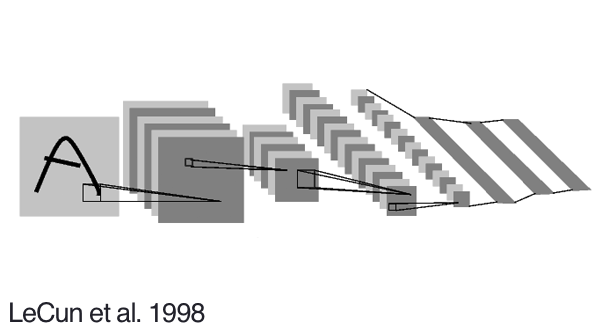
\includegraphics[width=\textwidth]{./imagenes/lenet.png}
\end{figure}

\subsection{Convolutional Layer}

En estas capas se aplica una operación de convolución a la entrada y el resultado es pasado a la siguiente capa. La operación de convolución emula la respuesta de una neurona individual ante un estímulo visual. Los parámetros de una red convolucional se componen de una serie de filtros que se aprenden. Cada filtro es pequeño, pero se extiende a lo largo de toda la profundidad de la entrada, en este caso una imagen. Esto quiere decir que si el filtro es 5x5 y la imagen es de 50x50, iremos pasando el filtro por cuadrados de 5x5 de la imagen hasta haberla recorrido en su totalidad.\\

Entonces, la red aprenderá filtros que se activen cuando vean cierto tipo de característica, como por ejemplo una esquina. Tendremos un filtro por neurona, por lo que habrá tantos filtros como neuronas tenga la capa de convolución.\\

\begin{figure}[H]
	\centering
	\caption{Ejemplo de filtros aprendidos por parte de Krizhevsky et al.}
    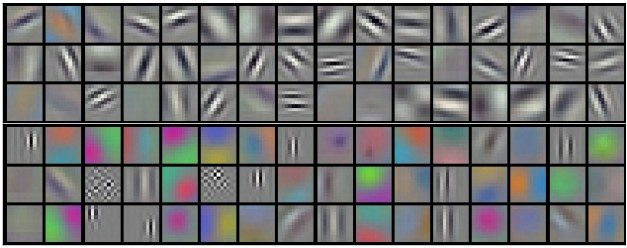
\includegraphics[width=\textwidth]{./imagenes//weights.jpeg}
\end{figure}

\subsection{Pooling Layer}
Es bastante normal insertar una capa de pooling entre sucesivas capas convolucionales. La función de una capa de pooling es reducir progresivamente el tamaño espacial de la representación para reducir la cantidad de parámetros y la computación en la red, y ayuda también para el control del overfitting. La capa de pooling opera independientemente en cada porción de profundidad de la entrada y le cambia el tamaño espacialmente, usando la operación de MAX. Lo que esto implica es que cada vez que aplicamos una capa de pooling, vamos reduciendo el tamaño espacial de la imagen.\\

Un ejemplo. Si tenemos una imagen de 224x224 y utilizamos una capa de pooling de 2x2, a la salida de esa capa, nuestra imagen, o mejor dicho la representación de la misma dentro de la red, tendrá un tamaño de 112x112, ya que la hemos reducido a la mitad con la operación de pool. Con la operación de MAX, lo que hacemos es que nos quedamos con el valor del máximo dentro de un grupo de píxeles.\\

\begin{figure}[H]
	\centering
	\caption{Ejemplo de capa de pool.}
    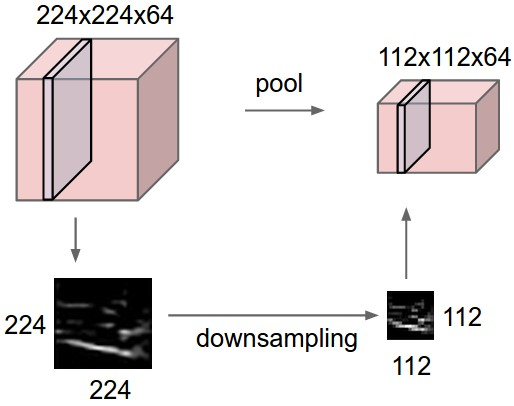
\includegraphics[width=\textwidth]{./imagenes/pool.jpeg}
\end{figure}
\begin{figure}[H]
	\centering
	\caption{Ejemplo de la operación maxpool.}
    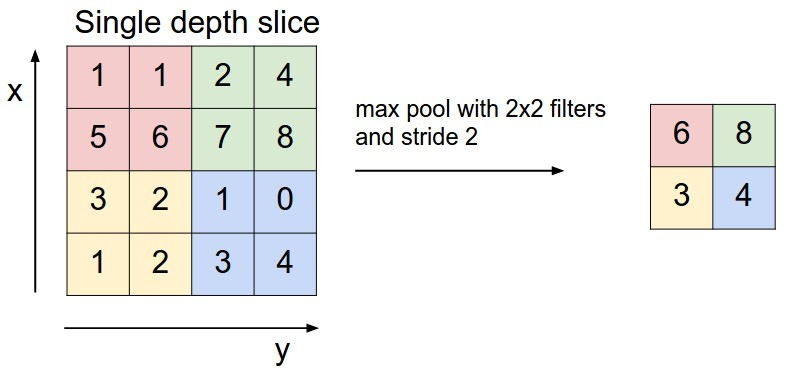
\includegraphics[width=\textwidth]{./imagenes/maxpool.jpeg}
\end{figure}

\subsection{Funciones de activación}

Como se ha explicado en la sección de las redes neuronales \ref{RedesNeuronales}, podemos tener distintas funciones de activación. Estas, definen la salida de la neurona dependiendo de cuál ha sido la entrada.\\

En nuestro caso usamos dos funciones de activación. Una es la función conocida como ReLU(Rectified Linear Unit) y la otra es la función conocida como Softmax.
\begin{figure}[H]
	\centering
	\caption{Función de activación Softmax}
	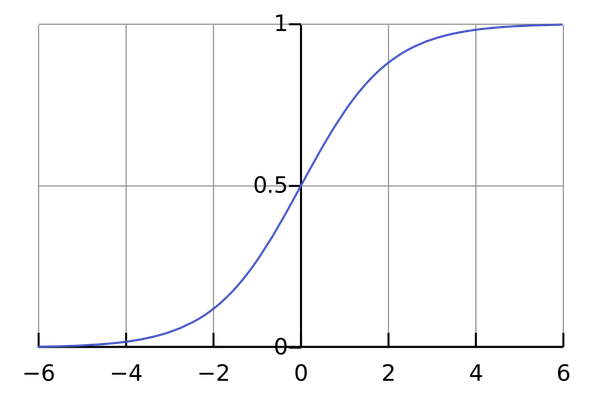
\includegraphics[height=300px,width=400px]{./imagenes/softmax.png}
\end{figure}
\newpage
\begin{figure}[H]
	\centering
	\caption{Función de activación ReLU}
	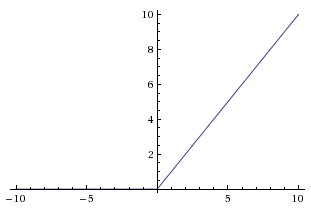
\includegraphics[height=300px,width=400px]{./imagenes/relu.jpg}
\end{figure}

La función de activación Softmax es la que se utilizará a la salida de la CNN para que nos de un valor de predicción. En el caso de que este valor sea 0, se clasificará la imagen como AD, y en el caso de que sea 1 se clasificará como Normal.\\

\section{Métodos de validación de modelos}

Para la validación del modelo empleado se han utilizado dos métodos, los cuáles son \textit{K-Fold cross-validation} y el \textit{Leave-one-out cross-validation}, que a continuación serán explicados brevemente.\\

\subsection{K-Fold Cross-Validation}

En el \textit{K-Fold Cross-Validation} se realiza una partición aleatoria del conjunto de datos en K partes. Entonces, se utilizará uno de estos subconjuntos para \textit{test} y los k-1 subconjuntos restantes se utilizarán para \textit{training}. Esto se repite K veces, sin repetir un subconjunto en \textit{test}. Entonces, se obtiene una media de los resultados en \textit{test} y con esto podemos hacernos una idea de como funciona nuestro modelo y de si generalizará bien. Esto incrementa el tiempo de entrenamiento y comprobación, por lo que no es un método muy usado en los los conjuntos de datos cuyo tamaño es muy grande, pero es de gran ayuda en conjuntos de datos más pequeños lo que nos permite validar mejor como será la generalización del modelo.\\

\begin{figure}[H]
	\centering
	\caption{Ejemplo de Cross Validation con K=4 \cite{k-fold}}
	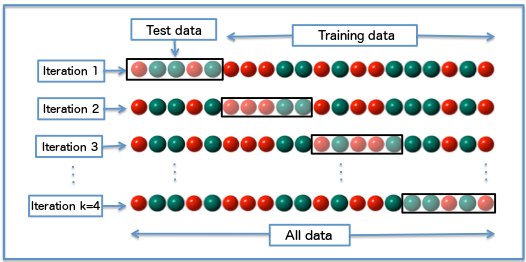
\includegraphics[width=\textwidth]{./imagenes/K-fold.jpg}
\end{figure}

\subsection{Leave-one-out Cross-Validation}
Este método podría ser un tipo de \textit{K-Fold cross-validation} en el que K es igual al número de elementos dentro del conjunto de datos. Esto implica que el tiempo de validación sea muy alto, ya que vamos a realidar K entrenamientos y K evaluaciones, pero es un método muy robusto para la validación del modelo.

\begin{figure}[H]
	\centering
	\caption{Ejemplo de  \textit{Leave one out Cross Validation} \cite{LOO}}
	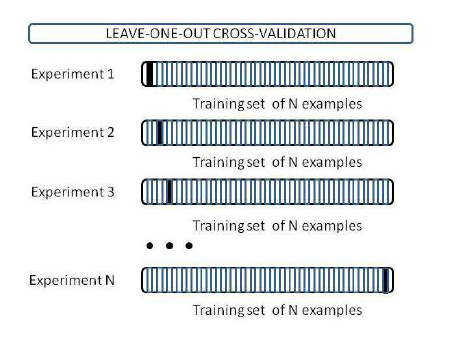
\includegraphics[width=\textwidth]{./imagenes/LOO.png}
\end{figure}
